Consider a dataset consisting of points in the form of $(x, y)$, where $x$ is a real value, and $y \in \{-1,\ 1\}$ is the class label. There are only three points $(x_1, y_1) = (-1,\ -1),\  (x_2, y_2) = (1, -1)$, and $(x_3, y_3) = (0,\ 1)$, shown in Figure~\ref{line_plot1}.

\vspace{0.3cm}
\begin{figure}[htbp] 
	\centering
	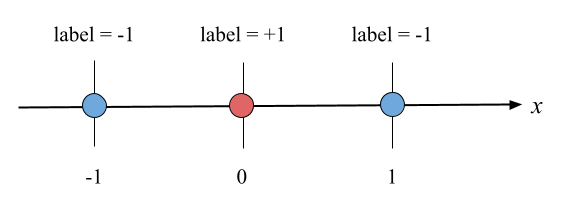
\includegraphics[width = .6\textwidth]{svm_line.png}
	\caption{Three data points considered in Problem 1}
	\label{line_plot1}
\end{figure}

\textbf{1.1} (\blue{2pts}) Can these three points in their current one-dimensional feature space be perfectly separated with a linear classifier? Why or why not?\\

\textbf{1.2} (\blue{3pts}) Now we define a simple feature mapping $\mathbf{\phi}(x) = [x, x^2]^T$ to transform the three points from one-dimensional to two-dimensional feature space. Plot the transformed points in the new two-dimensional feature space. Is there a linear model $\w^T\x +b$ for some $\w\in \R^2$ and $b \in \R$ that can correctly separate the three points in this new feature space? Why or why not?\\

\textbf{1.3} (\blue{2pts}) Given the feature mapping $\mathbf{\phi}(x) = [x, x^2]^T$, write down the $3 \times 3$ kernel/Gram matrix $\mathbf{K}$ for this
dataset.\\

\textbf{1.4} (\blue{4pts}) Now write down the primal and dual formulations of SVM for this dataset
in the two-dimensional feature space.
Note that when the data is separable, we set the hyperparameter $C$ to be $+\infty$
which makes sure that all slack variables ($\xi$) in the primal formulation have to be $0$
(and thus can be removed from the optimization).\\

\textbf{1.5} (\blue{5pts}) Next, solve the dual formulation exactly (note: while this is not generally feasible, the simple form of this dataset makes it possible).
Based on that, calculate the primal solution.\\

\textbf{1.6} (\blue{3pts}) Plot the decision boundary (which is a line) of the linear model ${\w^*}^T \x + b^*$ in the two-dimensional feature space, where $\w^*$ and $b^*$ are the primal solution you got from the previous question. Then circle all support vectors. Finally, plot the corresponding decision boundary in the original one-dimensional space (recall that the decision boundary is just the set of all points $x$ such that ${\w^*}^T \mathbf{\phi}(x) + b^* = 0$).\\
